%-----------------------------------------------------------------------------
%
%               Template for sigplanconf LaTeX Class
%
% Name:         sigplanconf-template.tex
%
% Purpose:      A template for sigplanconf.cls, which is a LaTeX 2e class
%               file for SIGPLAN conference proceedings.
%
% Guide:        Refer to "Author's Guide to the ACM SIGPLAN Class,"
%               sigplanconf-guide.pdf
%
% Author:       Paul C. Anagnostopoulos
%               Windfall Software
%               978 371-2316
%               paul@windfall.com
%
% Created:      15 February 2005
%
%-----------------------------------------------------------------------------

\documentclass{sigplanconf}

% The following \documentclass options may be useful:

% preprint      Remove this option only once the paper is in final form.
% 10pt          To set in 10-point type instead of 9-point.
% 11pt          To set in 11-point type instead of 9-point.
% authoryear    To obtain author/year citation style instead of numeric.

\usepackage{tikz}
\usepackage{amsmath}
\usepackage{graphicx}
\usepackage{xspace}
\usepackage{hyperref}
\hypersetup{
    bookmarks=false,        % show bookmarks bar?
    unicode=false,          % non-Latin characters in Acrobat’s bookmarks
    pdftoolbar=true,        % show Acrobat’s toolbar?
    pdfmenubar=true,        % show Acrobat’s menu?
    pdffitwindow=false,     % window fit to page when opened
    pdfstartview={FitH},    % fits the width of the page to the window
    pdftitle={My title},    % title
    pdfauthor={Author},     % author
    pdfsubject={Subject},   % subject of the document
    pdfcreator={Creator},   % creator of the document
    pdfproducer={Producer}, % producer of the document
    pdfkeywords={keyword1} {key2} {key3}, % list of keywords
    pdfnewwindow=true,      % links in new window
    colorlinks=true,        % false: boxed links; true: colored links
    linkcolor=black,        % color of internal links (change box color with linkbordercolor)
    citecolor=black,        % color of links to bibliography
    filecolor=black,        % color of file links
    urlcolor=black          % color of external links
}
% \usepackage{acronym}

%% macros
% \def \JCP{\ac{JCP}\xspace}
% \def \SUN{\mbox{Sun Microsystems}\xspace}
% \def \ORACLE{\mbox{Oracle}\xspace}
% \def \DALVIK{\mbox{Dalvik}\xspace}
% \def \Jsr{\ac{JSR}\xspace}
% \def \JSR{\Jsr 292\xspace}
% \def \GOOGLE{\mbox{Google}\xspace}
% \def \ANDROID{\mbox{Android}\xspace}
% \def \JVM{\ac{JVM}\xspace}
% \def \DEX{\mbox{DEX}\xspace}
% \def \VM{\ac{VM}\xspace}
% \def \BSM{\ac{BSM}\xspace}
\def \JCP{JCP\xspace}
\def \SUN{\mbox{Sun Microsystems}\xspace}
\def \ORACLE{\mbox{Oracle}\xspace}
\def \DALVIK{\mbox{Dalvik}\xspace}
\def \Jsr{JSR\xspace}
\def \JSR{\Jsr 292\xspace}
\def \GOOGLE{\mbox{Google}\xspace}
\def \ANDROID{\mbox{Android}\xspace}
\def \JVM{JVM\xspace}
\def \DEX{\mbox{DEX}\xspace}
\def \VM{VM\xspace}
\def \BSM{BSM\xspace}

\newcommand{\executeiffilenewer}[3]{%
  \ifnum\pdfstrcmp{\pdffilemoddate{#1}}{\pdffilemoddate{#2}}>0%
  {\immediate\write18{#3}}\fi%
}

\newcommand{\includesvg}[1]{%
  \executeiffilenewer{#1.svg}{#1.pdf}{inkscape -z -D --file=#1.svg --export-pdf=#1.pdf --export-latex}%
  \input{#1.pdf_tex}%
}

\begin{document}

\special{papersize=8.5in,11in}
\setlength{\pdfpageheight}{\paperheight}
\setlength{\pdfpagewidth}{\paperwidth}

\conferenceinfo{PPPJ '14}{Month d--d, 20yy, City, ST, Country} 
\copyrightyear{2014} 
\copyrightdata{978-1-nnnn-nnnn-n/14/mm} 
\doi{nnnnnnn.nnnnnnn}

% Uncomment one of the following two, if you are not going for the 
% traditional copyright transfer agreement.

%\exclusivelicense                % ACM gets exclusive license to publish, 
                                  % you retain copyright

%\permissiontopublish             % ACM gets nonexclusive license to publish
                                  % (paid open-access papers, 
                                  % short abstracts)

\titlebanner{banner above paper title}        % These are ignored unless
\preprintfooter{short description of paper}   % 'preprint' option specified.

\title{Title Text}
\subtitle{Subtitle Text, if any}

\authorinfo{Roussel Gilles}
           {University Paris-Est Marne-la-Vallee}
           {roussel@univ-mlv.fr}
\authorinfo{Forax Remi}
           {University Paris-Est Marne-la-Vallee}
           {forax@univ-mlv.fr}
\authorinfo{Pilliet Jerome}
           {University Paris-Est Marne-la-Vallee}
           {pilliet@univ-mlv.fr}

\maketitle

\begin{abstract}
This is the text of the abstract.

bla bla bla bla bla bla bla bla bla
bla bla bla bla bla bla bla bla bla
bla bla bla bla bla bla bla bla bla
bla bla bla bla bla bla bla bla bla
bla bla bla bla bla bla bla bla bla
bla bla bla bla bla bla bla bla bla
bla bla bla bla bla bla bla bla bla
\dots
\end{abstract}

\category{CR-number}{subcategory}{third-level}

% general terms are not compulsory anymore, 
% you may leave them out
\terms
term1, term2

\keywords
keyword1, keyword2

  \section{Android}

    \ANDROID is the mobile operating system of Google.
    It's an open-source project called ``\ANDROID Open-Source Project'' (AOSP).
    In Q2 2013, \ANDROID occupies almost 80\% of the market share with more than 187 million units shipped \cite{idc-website}.
    The success of \ANDROID can be explain by an open project and an open market
    which are very attractive for devices producers, service providers and application developers \cite{ieee-butler-android-landscape}.
%     \ANDROID est l'OS mobile de Google.
%     C'est un projet open-source appel\'e ``\ANDROID Open-Source Project'' (AOSP).
%     Au 2\`eme trimestre 2013, \ANDROID occupe pr\`es de 80\% de part de march\'e avec plus de 187 millions d'unit\'es livr\'ees.

    \ANDROID mainly run on embedded environments like smartphones and tablets.
    Therefore, strong constraints apply to \ANDROID
    and it have to support ARM architecture and now Intel architecture.
%     \ANDROID tourne principalement sur des environnements embarqu\'es tels que les t\'el\'ephones portables et les tablettes tactiles.
%     De ce fait, des contraintes fortes s'appliquent \`a \ANDROID.
%     Il doit donc supporter les architectures ARM m\^eme si les architectures Intel commencent \`a arriver.
    
    Even if hardware of devices which supports \ANDROID becomes more efficient,
    devices can't be as efficient as a desktop computer because of miniaturization of devices.
    Being a mobile device requires a minimal energetic consumption.
    Moreover, \ANDROID is portable and it must be adaptable to different devices.
    Forcing it to abstract itself from hardware.
%     Meme si le materiel des appareils supportant \ANDROID devient de plus en plus performant,
%     la miniaturisation des appareils fait qu'ils ne peuvent pas \^etre aussi performant que les ordinateurs.
%     Le fait d'\^etre sur de machine mobile demande aussi une consommation energ\'etique minimale.
%     De plus, \ANDROID est portable et doit pouvoir s'adapter \`a differents appareils.
%     Ce qui l'oblige \`a s'abstraire du materiel.

    \begin{figure}
      \centering
      \def\svgwidth{\columnwidth}
      \includesvg{android-system-architecture}
      \caption{android system architecture \cite{wiki-android}}
      \label{ASA}
    \end{figure}

    The \ANDROID architecture is described like a ``software stack'' (fig. \ref{ASA}).
    It's composed to:
%     Il est descrit comme \'etant une ``pile de logiciels'' (software stack) (fig. \ref{ASA}).
%     Cette \emph{pile} se compose
    \begin{itemize}
      \item a modified version of the Linux kernel.
        It offers an hardware abstraction,
        an existing memory and process managements
        and a security and networking models;
      \item native libraries (C/C++)
        which provide most of features of the \ANDROID system;
      \item a virtual machine called ``\DALVIK''. \DALVIK is a important component of \ANDROID.
        It runs applications converted into the \DEX format.
        \DALVIK uses a core API written from scratch in Java
        which can be assimilate to the version 5 or 6 of the Java API;
      \item an application framework to enable the making of \ANDROID applications;
      \item and some default applications.
%      \item d'un noyau linux modifi\'e;
%      \item d'un ensemble de biblioth\'eques \'ecrites en C/C++;
%      \item d'une machine virtuelle (\DALVIK) et d'une API \'ecrite en Java;
%      \item d'un framework pour concevoir des applications.
%      \item ainsi que d'une suite d'applications par d\'efaut.
    \end{itemize}

    \subsection{Differences between the JVM and Dalvik}

      \begin{figure}[h]
        \centering
        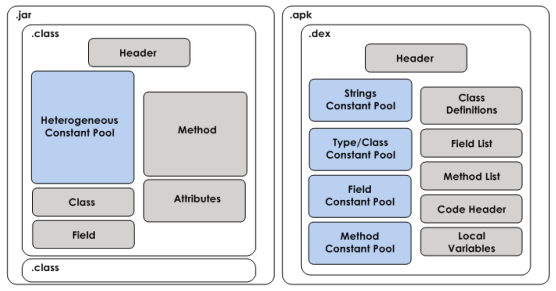
\includegraphics[width=\columnwidth]{structure-jar-apk.png}
        \caption{structure of JAR and APK files}
        \label{SJA}
      \end{figure}

      The main difference between these two machines is that \DALVIK is a register based machine while the \JVM is stack based.
      A stack based VM uses more instructions to manipulate data and to implement Java code than a register based VM.
      But the register based VM instructions tends to be larger \cite{ieee-paul-kundu-energy-perspective}

      The bytecode Java is given in a ``.class'' file and only contains the code of one class (fig. \ref{SJA}).
      The file is made of a series of tables, which contains various information, the code of the class and some other things.
      The code contains references to these tables.
      Among these tables, one is the table of constants (constant-pool).
      This table stores most of the constant values of the class (numbers or texts)
      and more evolved elements (data types, class names, attribute names, \dots).
%       Le format compil\'e du code Java est donn\'e dans un fichier ``.class'' et ne contient le code que d'une seule classe.
%       Ce fichier contient entre autre, une suite de tables contenant diverses informations et le code de la classe.
%       Le code contient des r\'ef\'erences vers ces tables.
%       Parmis ces tables, il y a la table des constantes (contants-pool).
%       La table des constantes stocke la plupart des valeurs constantes dans la classe (nombres ou textes)
%       ainsi que d'\'el\'ements plus \'evolu\'es (types de donn\'ees, noms de classes, noms d'attributs, ...).

      Whereas, \DEX format contains all the code of the application (fig. \ref{SJA}).
      It will be loaded in one piece.
      It is a read-only format, so the code can't be changed at runtime.
      Duplicate constants such as strings used in multiple class files
      are included only once in the \DEX file to save space.
      Unlike the \JVM, \DALVIK uses one constant-pool by type of constant
      except for the primitive types which are directly encoded with the opcode.\\

      \begin{figure}[h]
        \centering
        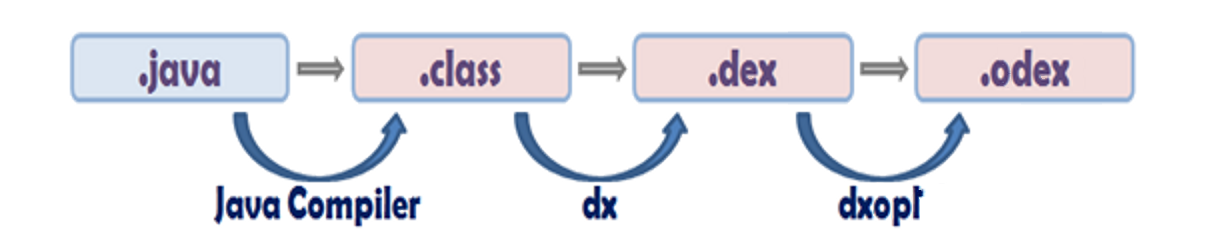
\includegraphics[width=\columnwidth]{dex-tools-chain.png}
        \caption{\ANDROID application tools-chain}
        \label{DTC}
      \end{figure}

      \DALVIK cannot directly execute Java bytecode.
      It have first to translate the Java byte code to a \DALVIK specific bytecode called \DEX
      and It cans optimize its bytecode (\mbox{ODEX}) to save space (fig. \ref{DTC}).

  \section{Java Specification Request 292}

    The \JSR is a request from \JCP and led by \SUN in 2006.
    It had been integrated in 2011 in the version 7 of Java,
    modifying both the Java language specification and the \JVM specification.

    Since late 90's, a lot of language
    implementors have chosen the JVM as their target platform \cite{wiki-jvm-lang},
    for several reasons among the size of the ecosystem,
    the presence of mature GCs and Just In Time compilers. 

    The aim of this \Jsr is to ease the implementation of dynamically typed languages
    by providing a new way to do function calls that allows language implementors
    to specify a specific semantics, independantly of the semantics of the language Java.
    
    This \Jsr is composed of two parts, the first part, specifies the semantics of
    new opcodes. The second part defined an API, java.lang.invoke that allows
    to create runtime typesafe function pointers (java.lang.invoke.MethodHandle) and
    methods to combine those function pointers to do thing like function composition,
    function argument permutation, etc.

    The next sections will present the new API and new instructions but before
    we want to introduce an example that we will use for the rest of the paper.

    \subsection{Example}
      Let suppose we have the following code in Groovy \cite{lang-groovy}
      
      {\tiny      
      \begin{verbatim}
  def foo(a) {
    a + 2
  }

  println foo(9)
  println foo("test")
      \end{verbatim}
      }

      It prints 11 and test2. For the fist call to foo, a is an integer so the function + refers
      to the function +(int,int) while for the second call to foo, a is a string, so the
      function + refers to the function +(String,String).

      If one try to translate that code in Java bytecode, it will be something like
      {\tiny      
      \begin{verbatim}
  def foo(a) {
    aload 0   // 0 is offset of first variable, 'a' here
    iconst_2  // load the integer constant 2
    invokevirtual Object + (I)LObject;
    areturn 
  }
      \end{verbatim}
      }

      As you can see, the Java bytecode is typed, each instruction is prefixed 
      by the type of the operand ('a' for object, 'i' for integer, etc)
      and the method call (invokevirtual) specify the type of the receiver and its parameter ;
      an object (java/lang/Object) followed by an int (I) ; and its return type
      which is also an object in the example.

      The code above doesn't work because invokevirtual is an existing Java bytecode that call
      a virtual method using the Java semantics so the Virtual Machine or more precisely
      the bytecode verifier will check that there is a method '+' on java.lang.Object
      that takes an int and return an Object. If you have used Java, you alreadty know
      that this method doesn't exist. So the bytecode verification will fail. 

      Another possible translation is to use a cascade of if ... instanceof.
      {\tiny      
      \begin{verbatim}
  static Object plus(String v, Object v2) {
    return v.concat(String.valueOf(v2));
  }

  static Object plus(int v, int v2) {
    return Integer.sum(v, v2)
  }

  static Object foo(Object v, int i) {
    if (v instanceof Integer) {
      return plus((Integer)v, i);
    }
    if (v instanceof String) {
      return plus((String)v, i);
    }
    throw new Error();
  }

  public static void main(String[] args) {
    System.out.println(foo(9));
    System.out.println(foo("bar"));
  }
      \end{verbatim}
      }

      While this code works, it supposes that all possible variations of + are known at compile time,
      something which is not true in most dynamic languages (Ruby, Groovy, Dart by example).
      This code can also be slow because for real languages, the number of if ... instanceof branches
      can be greater than a dozen. 
      
      To solve these issues, the \Jsr introduces a new bytecode named invokedynamic with no predefined
      linking semantics and a mechanism that allows to specify the linking semantics in Java
      or any languages that can be compiled to bytecodes.
      Invokedynamic is a function call so it can simulate every other existing Java calls that delegate
      its linking semantics to an external Java method, the bootstrap method.
      The bootstrap method is called the first time the invokedynamic opcode is encounter by the interpreter,
      with the context where the opcode is located i.e.
      the declaring class (encapsulated in a java/lang/invoke/Lookup object), a symbolic name,
      the declared parameter types as a java/lang/invoke/MethodType and return
      a CallSite object which is a box that contains a function pointer (a java/lang/MethodHandle).
      Any subsequent execution of the invokedynamic opcode will call the function pointer
      stored inside the callsite object returned by the bootstrap method.
      
      For our running example, the code of foo with invokedynamic is
     {\tiny      
      \begin{verbatim}
  def foo(a) {
    aload 0
    iconst_2 
    invokedynamic  + (LObject;I)LObject;
      bsm: invokestatic RT.bootstrap:(LMethodHandles$Lookup;LString;LMethodType;)LCallSite;
    areturn 
  }
      \end{verbatim}
      }

      The first time that foo is executed, the method bootstrap of the class RT will be called, with a lookup corresponding to the class containing foo,
      "+" as string and a MethodType corresponding to the descriptor "(Ljava/lang/Object;I)Ljava/lang/Object;".
      The implementation of the method bootstrap is able to create lazily a code shape similar to the tree of test if ... instanceof,
      we have seen above by creating method handles (function pointers) that can be organized as a tree. 
      
      So invokedynamic allows to separate the code of a dynamic language in two parts, a static part which is compiled directly to JVM bytecode
      and a dynamic part which is specified by a tree of method handles.
      The way to create a tree of method handles is to use the package java.lang.invoke.      


      
      \begin{figure}
        % graph 1
        \centering \resizebox{.6\linewidth}{!}{%
          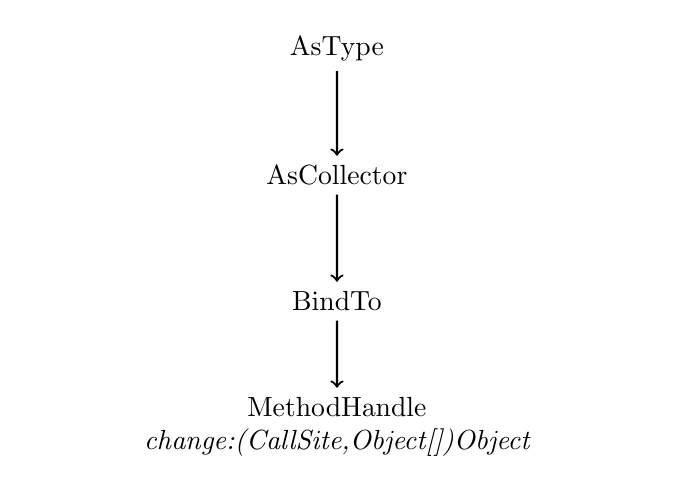
\begin{tikzpicture}[scale=1.6]
            \node[text width=3in,align=center](A1) at (2,-2){AsType};
            \node[text width=3in,align=center](A2) at (2,-3){AsCollector};
            \node[text width=3in,align=center](A3) at (2,-4){BindTo};
            \node[text width=3in,align=center](A4) at (2,-5){MethodHandle\\{\it change:(CallSite,Object[])Object}};

            \draw[thick,->](A1) -- (A2);
            \draw[thick,->](A2) -- (A3);
            \draw[thick,->](A3) -- (A4);
          \end{tikzpicture}
        }
        \caption{}
      \end{figure}

      \begin{figure}
        % graph 2
        \centering \resizebox{\linewidth}{!}{%
          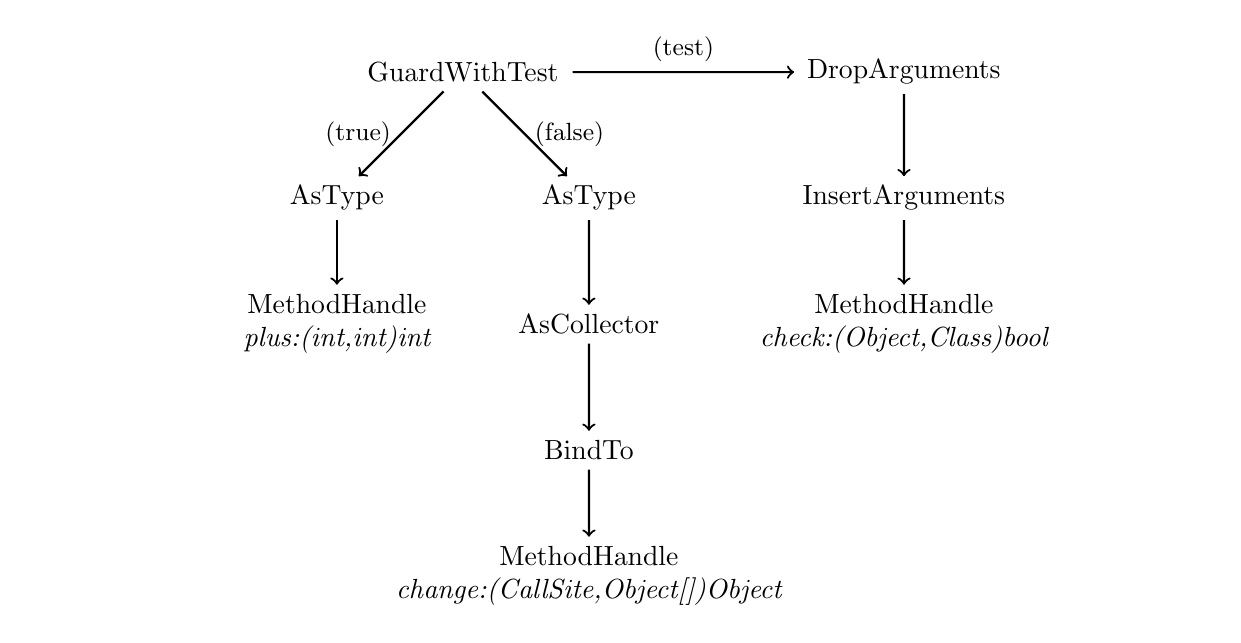
\begin{tikzpicture}[scale=1.6]
            \node[text width=3in,align=center](A1) at (2,-2){AsType};
            \node[text width=3in,align=center](A2) at (2,-3){AsCollector};
            \node[text width=3in,align=center](A3) at (2,-4){BindTo};
            \node[text width=3in,align=center](A4) at (2,-5){MethodHandle\\{\it change:(CallSite,Object[])Object}};

            \node[text width=1in,align=center](G1) at (1,-1){GuardWithTest};

            \node[text width=3in,align=center](B1) at (0,-2){AsType};
            \node[text width=3in,align=center](B2) at (0,-3){MethodHandle\\{\it plus:(int,int)int}};

            \node[text width=1in,align=center](C1) at (4.5,-1){DropArguments};
            \node[text width=3in,align=center](C2) at (4.5,-2){InsertArguments};
            \node[text width=3in,align=center](C3) at (4.5,-3){MethodHandle\\{\it check:(Object,Class)bool}};

            \draw[thick,->](A1) -- (A2);
            \draw[thick,->](A2) -- (A3);
            \draw[thick,->](A3) -- (A4);
            \draw[thick,->](B1) -- (B2);

            \draw[thick,->](C1) -- (C2);
            \draw[thick,->](C2) -- (C3);
            \draw[thick,->](G1) -- node[right] {\small (false)} (A1);
            \draw[thick,->](G1) -- node[left]  {\small (true)}  (B1);
            \draw[thick,->](G1) -- node[above] {\small (test)}  (C1);
          \end{tikzpicture}
        }
        \caption{}
      \end{figure}

      \begin{figure*}
        % graph 3
        \centering
        \resizebox{.8\linewidth}{!}{%
          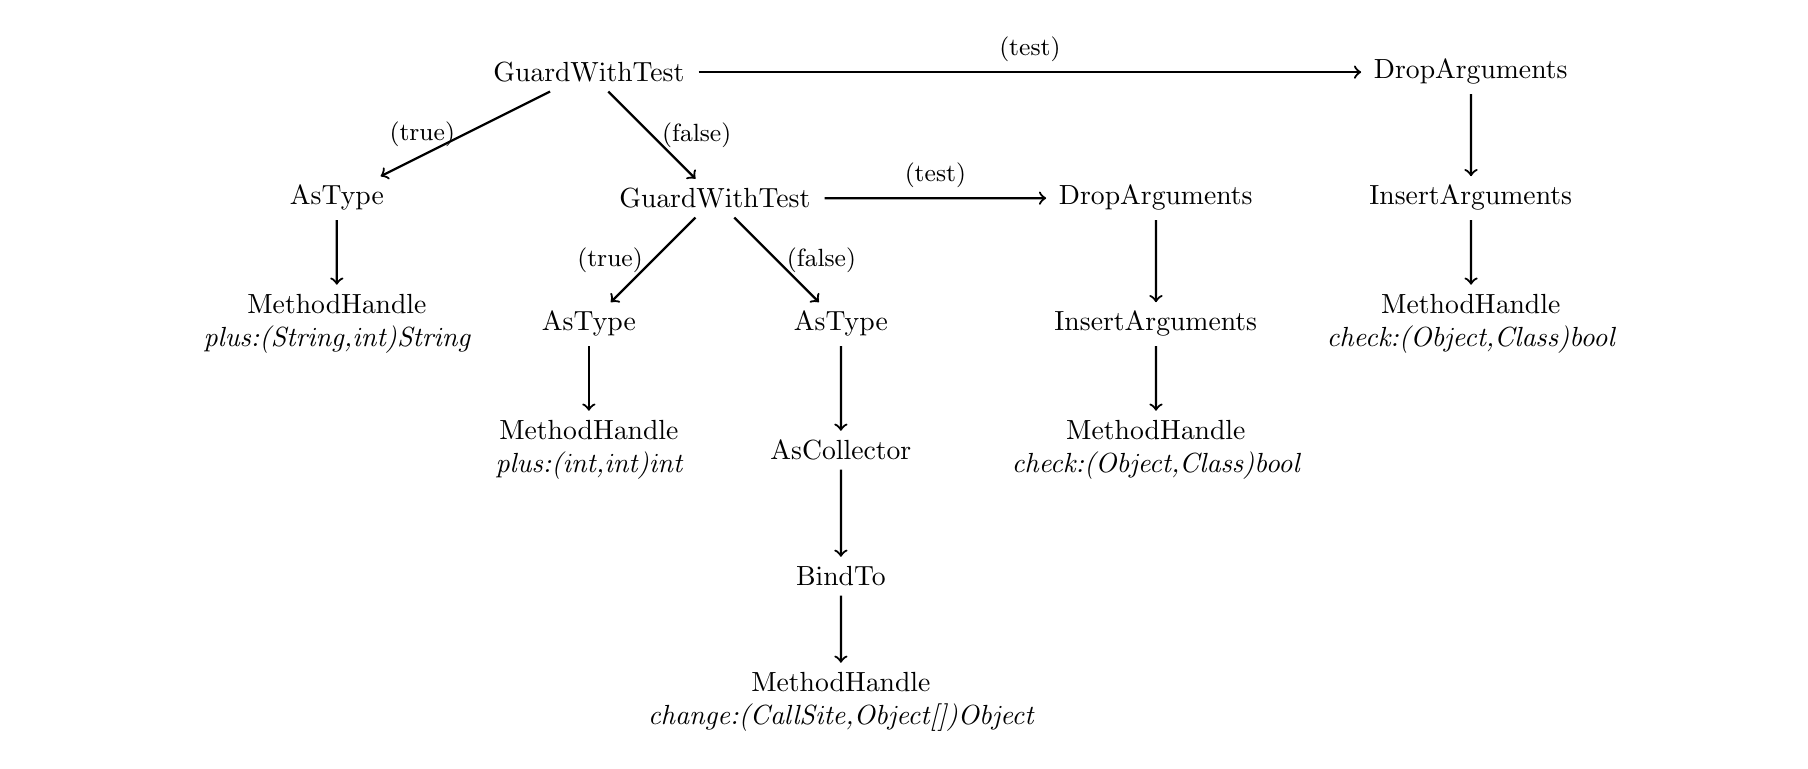
\begin{tikzpicture}[scale=1.6]
              \node[text width=3in,align=center](A1) at (2,-2){AsType};
              \node[text width=3in,align=center](A2) at (2,-3){AsCollector};
              \node[text width=3in,align=center](A3) at (2,-4){BindTo};
              \node[text width=3in,align=center](A4) at (2,-5){MethodHandle\\{\it change:(CallSite,Object[])Object}};

              \node[text width=1in,align=center](G1) at (1,-1){GuardWithTest};

              \node[text width=3in,align=center](B1) at (0,-2){AsType};
              \node[text width=3in,align=center](B2) at (0,-3){MethodHandle\\{\it plus:(int,int)int}};

              \node[text width=1in,align=center](C1) at (4.5,-1){DropArguments};
              \node[text width=3in,align=center](C2) at (4.5,-2){InsertArguments};
              \node[text width=3in,align=center](C3) at (4.5,-3){MethodHandle\\{\it check:(Object,Class)bool}};

              \node[text width=1in,align=center](G2) at (0, 0){GuardWithTest};

              \node[text width=3in,align=center](D1) at (-2,-1){AsType};
              \node[text width=3in,align=center](D2) at (-2,-2){MethodHandle\\{\it plus:(String,int)String}};

              \node[text width=1in,align=center](E1) at (7, 0){DropArguments};
              \node[text width=3in,align=center](E2) at (7,-1){InsertArguments};
              \node[text width=3in,align=center](E3) at (7,-2){MethodHandle\\{\it check:(Object,Class)bool}};

              \draw[thick,->](A1) -- (A2);
              \draw[thick,->](A2) -- (A3);
              \draw[thick,->](A3) -- (A4);
              \draw[thick,->](B1) -- (B2);

              \draw[thick,->](C1) -- (C2);
              \draw[thick,->](C2) -- (C3);
              \draw[thick,->](G1) -- node[right] {\small (false)} (A1);
              \draw[thick,->](G1) -- node[left]  {\small (true)}  (B1);
              \draw[thick,->](G1) -- node[above] {\small (test)}  (C1);

              \draw[thick,->](D1) -- (D2);
              \draw[thick,->](E1) -- (E2);
              \draw[thick,->](E2) -- (E3);
              \draw[thick,->](G2) -- node[right] {\small (false)} (G1);
              \draw[thick,->](G2) -- node[left]  {\small (true)}  (D1);
              \draw[thick,->](G2) -- node[above] {\small (test)}  (E1);
          \end{tikzpicture}
        }
        \caption{}
      \end{figure*}

      \subsection{Package java.lang.invoke}

      The \JSR has created a new package named ``java.lang.invoke''.
      It contains several classes to ease the implementation of dynamic languages support.
      These classes are directly understood by the \JVM.
      It is composed of classes MethodType, MethodHandle, CallSite and SwitchPoint.
      All classes answer to one or more problems coming from dynamic languages optimizations or implementations.



      \subsubsection{MethodHandle}
        A method handle is a runtime type checked, directly executable reference to
        either an underlying method, constructor, field, or similar low-level operation,
        or to a combiner operation that takes one or more method handles as input and
        applies an operation like an argument transformation, a function compositions, etc.
        The former kind of method handle is called a direct method handle,
        the later is called a combiner method handle.
        
        To guarantee runtime type safety, any method handle embodies a method type (of type java.lang.invoke.MethodType)
        that describe the parameter types and the return type that a method handle accept.
        When a method handle is called, the method type is checked using different semantics depending on the
        kind of call.

        There are two kind of method handle call semantics. 
        \begin{itemize}
          \item the exact call semantics, in that case, the declared type of the arguments (and return value) at a call site
                must be exactly the same as the types of the method type.
          \item the generic call semantics, in that case, the arguments can be converted using widening primitive conversions,
                boxing and unboxing conversions and varargs conversions as defined in the Java Language Specification.
        \end{itemize}
        None of these semantics implement the calling semantics as defined by the Java Virtual Machine Specification
        for classical Java method calls like invokestatic or invokevirtual
        \footnote{There is also a minor difference between the generic call semantics and the call semantics of
         the Java Language Specification if the method is a varargs and the call as the same number of parameters as the method.
         The generic call semantics will not try to do the varargs conversion if the last parameter is not an array.},
        the exact call semantics is more strict, and the generic call semantics is more permissive.

        


      \subsubsection{MethodType}
        A method type represents the arguments and return type accepted and returned by a method handle,
        or the arguments and return type passed and expected by a method handle caller.
        This class represents a method signature.
        A method type is immutable, so this type can be created only by factory methods.
        
%         All instances of MethodType created by \DALVIK are not interned,
%         all others are interned into a Java structure.

        {\tiny
          \begin{verbatim}
    // "bar".concat(String.valueOf(2));
  MethodType.methodtype(String.class,String.class);

    // Integer.sum(a, 2);
  MethodType.methodtype(int.class,int.class,int.class);
          \end{verbatim}
        }

      

      \subsubsection{CallSite}
        A CallSite is a holder for a variable MethodHandle, which is called its target.
        An invokedynamic instruction linked to a CallSite delegates all calls to the site's current target.
        A CallSite may be associated with several invokedynamic instructions,
        or it may be "free floating", associated with none.\\

        It has three immediate, concrete subclasses that may be either instantiated or subclassed.
        \begin{enumerate}
          \item \textbf{ConstantCallSite} : If a mutable target is not required.
          \item \textbf{MutableCallSite}  : If a mutable target is required
          \item \textbf{VolatileCallSite} : If a mutable target is required which has volatile variable semantics.
        \end{enumerate}
        A non-constant call site may be relinked by changing its target.
        The new target must have the same type as the previous target.

      \subsubsection{SwitchPoint}
        The Java bytecode is compiled and optimized on the fly by the JIT compiler.
        However, it may be that the code need to be deoptimize.
        The \JVM contains some ``flags'' which indicate a need to degrade a code.
        So, it can ``drop'' a optimized code to optimize it again.
        it is essential that all threads were aware of changes.
        Using the safe-point (a mechanism of Garbage Collector) is recommended.
          % Le bytecode Java est compil\'e et optimis\'e \`a la vol\'ee par JIT.
          % Il arrive cependant que le code est besoin d'\^etre d\'esoptimis\'e (to degrade).
          % La JVM dispose de ``flags'' lui indiquant si un bout de code doit \^etre d\'esoptimis\'e.
          % Elle peut alors ``jeter'' du code optimis\'e pour faire \`a nouveau les optimisations.
          % Il est primordial que toutes les threads soient au courant de cette modification.
          % Pour cela, l'utilisation du SavePoint (m\'ecanisme du Garbage Collector) est pr\'econis\'e.

        A SwitchPoint is an object allowing this mechanism.
        It indicates that a code must be degraded and synchronizes threads.
        The SavePoint is not necessarily available.
        An alternative is to synchronize all threads with a volatile variable.
        It contains a target method and a fallback method.
          % Un SwitchPoint est un objet permettant ce m\'ecanisme.
          % Il indique qu'un code doit \^etre d\'esoptimis\'e et synchronise les threads.
          % Si le SavePoint n'est pas accessible, on peut synchroniser les threads \`a l'aide d'une variable volatile.
          % Il contient une target et une fallback.
%         http://docs.oracle.com/javase/7/docs/api/java/lang/invoke/SwitchPoint.html
        
        
%     \subsubsection{MethodHandle}
%       \label{jsrMH}
%       A method handle is a typed, directly executable reference to
%       an underlying method, constructor, field, or similar low-level operation,
%       with optional transformations of arguments or return values.
% 
% 
%       \begin{enumerate}[A.]
%         \item \textbf{Kinds of MethodHandle}\\
%           The MethodHandle class is composed of different types grouped into 4 kinds,
%           ``constant'', ``bound'', ``invokers'' and ``others''.
%           The three first have many specials paths in the \VM for each instruction.
%           While ``others'' have a unique path.
% 
%           \begin{enumerate}[1.]
%             \item \textbf{Constant}\\
%               The kind ``constant'' contains many instructions:\\
% 
%               \begin{tabular}{c c c}
%                 \begin{minipage}{4cm}
%                   \begin{itemize}
%                     \item invokeVirtual
%                     \item invokeInterface
%                     \item invokeStatic
%                     \item invokeSpecial
%                   \end{itemize}
%                 \end{minipage}
%                 &
%                 \begin{minipage}{4cm}
%                   \begin{itemize}
%                     \item getStatic
%                     \item putStatic
%                     \item getField
%                     \item putField
%                   \end{itemize}
%                 \end{minipage}
%                 &
%                 \begin{minipage}{5cm}
%                   \begin{itemize}
%                     \item invokeDirect (\DALVIK)
%                     \item newInvokeSpecial
%                   \end{itemize}
%                 \end{minipage}
%               \end{tabular}
% 
%             \item \textbf{Bound}\\
%               The kind ``bound'' contains an invoke-virtual \textit{un-virtualized}.
%               It is a MethodHandle constant created with invoke-virtual or invoke-interface
%               and a call to the ``bindTo'' function to bind the receiver.
%               It is equivalent to calling the Dalvik instructions :
%               \textit{invoke-direct} with a constant object on first parameter..
% 
%             \item \textbf{Invoker}
%               \begin{itemize}
%                 \item invoker
%                 \item ExactInvoker
%                 \item VarargCollectorInvoker (?)
%               \end{itemize}
% 
%             \item \textbf{And the others}\\
%               Those are MethodHandle adapters.
%           \end{enumerate}
% 
%         \item \textbf{Contents}\\
%           It contains a type descriptor (methodtype).
%           All instances of MethodHandle are immutable.
%           It have a pair of special invoker methods called invokeExact and invoke.
%           The invokeExact invoker accepts calls which exactly match the method handle's own type.
% 
%           \begin{enumerate}[1.]
%             \item \textbf{invokeExact method}\\
%               The invokeExact method allows to call a method handle with an exact type match.
%               The symbolic type descriptor at the call site of invokeExact
%               must exactly match this method handle's type.
%               No conversions are allowed on arguments or return values.
%               A runtime exception is thrown otherwise.
% 
%             \item \textbf{invoke method}\\
%               The invoke method allows to call a method handle
%               and eventually performing conversions on arguments and return values.
%               It's semantically equivalent to call a method named ``asType'' to convert the type descriptor.
%               This method thrown an ``ClassCastException'' if the conversion is impossible.
%               When the type descriptor and the method handle type descriptor correspond, it calls the invokeExact method.
%           \end{enumerate}
%       \end{enumerate}


    \subsection{Instructions}
      Even if formally the \JSR adds only one instruction to the opcode set (``invokedynamic''),
      it also enhances the semantics of the ldc (load constant) instructions to load two new constants.
      The \JSR add new instructions to the \VM opcode set like ``invokedynamic''.
      The ``ldc'' instruction has been enlarge to accept few new instructions.
      And some native methods are used as instructions.

      \subsubsection{ldc\_methodtype}
        Like classes and strings, method types can also be
        represented directly in a class file's constant pool as constants.
        A method type may be loaded by an ldc instruction which refers to a suitable
        CONSTANT\_MethodType constant pool entry.

      \subsubsection{ldc\_methodhandle}
        % TODO footnote 'polymorphic signature'
        Java code can create a constant native method with a polymorphic signature.
        A method handle that directly accesses any
        method, constructor, or field that is accessible to that code.
        Method handles that correspond to accessible fields, methods, and constructors
        can also be represented directly in a class file's constant pool
        as constants to be loaded by ldc bytecodes.

        A new type of constant pool entry, CONSTANT\_MethodHandle,
        refers directly to an associated CONSTANT\_Methodref,
        CONSTANT\_InterfaceMethodref or CONSTANT\_Fieldref constant pool entry.

      \subsubsection{invokedynamic}
        An invokedynamic instruction allows to call a method dynamically.

        Before the first call, It must be initialized with a bootstrap method.
        This bootstrap method can take 0 to 251 arguments.
        Then, a call site is produced and replaces the first call.
        Moreover, a bootstrap method may be only an invokeStatic or an newInvokeSpecial.

        It needs a descriptor of the resolved type of call, the target's name and a bootstrap method.

      \subsubsection{invokeVirtual on MH.invokeExact and MH.invoke}
        These instructions are here to make simple method calls\\
        \mbox{\textit{MethodHandle.invokeExact}} and \mbox{\textit{MethodHandle.invoke}}.
        Indeed, they are methods with a polymorphic signatures,
        so, it's difficult or impossible to implement it in Java.
        They use variables in the stack.
        The code cannot be more optimized than with a VM instruction.
          % Ces instructions sont l\`a pour simplifier les appels aux m\'ethodes MethodHandle.invokeExact et MethodHandle.invoke.
          % En effet, elles ont des signatures polymorphes, il est donc difficile voir impossible de les impl\'ementer en Java.
          % Ils utilisent les variables disponibles sur la pile.
          % Le code ne peut donc pas \^etre mieux optimis\'e qu'avec l'utilisation d'une instruction dans la VM.

  \subsection{Probl\`eme}

    \subsubsection{2 impl\'ementations (J9/HotSpot)}
    \subsubsection{Dalivk = VM sp\'ecifique}
    \subsubsection{non r\'eutilisation des techniques}
    \subsubsection{pas le m\^eme format DEX}

  \subsection{Solutions}

    \subsubsection{nouveau format DEX}
    \subsubsection{nouvelles fa\c cons d'impl\'ementations}

\section{Nouveau DEX}

  \subsection{opcodes / LDC}
  \subsection{DEX header (constant-pools)}
  \subsection{Class header}
  \subsection{r\'etro-compatibilit\'e}

\section{Impl\'ementations d'invoke-kind et des LDC}

  \subsection{LDC}

    \subsubsection{MethodType (intern\'e ou pas)}
    \subsubsection{MethodHandle}

  \subsection{invoke-generic}
  \subsection{invoke-exact}
  \subsection{invoke-dynamic}

    \subsubsection{tableau des MethodHandle (volatile)}
    \subsubsection{CAS (bootstrap)}

\section{Impl\'ementations des Combinateurs}

  \subsection{Impl\'ementation g\'en\'erale}
  \subsection{Quelques exemples (GWT, fold, ...)}

\section{Benchmark}  

\section{Related Work}

\section{Conclusion}


\appendix
\section{Appendix Title}

This is the text of the appendix, if you need one.

\acks

Acknowledgments, if needed.

% We recommend abbrvnat bibliography style.

\makeatletter
  \def\@seccntformat#1{Appendix~\csname the#1\endcsname:\quad}
\makeatother

%   \section{Acronyms}
%     \begin{acronym}[TDMA]
%       \acro{JCP}{Java Community Process}
%       \acro{VM}{Virtual Machine}
%       \acro{JVM}{Java Virtual Machine}
%       \acro{JSR}{Java Specification Request}
%       \acro{BSM}{Bootstrap Method}
%     \end{acronym}

\bibliographystyle{abbrvnat}

% The bibliography should be embedded for final submission.

\begin{thebibliography}{}
  \softraggedright

  \bibitem{idc-website}
  IDC website (2013) - \\ \url{www.idc.com/getdoc.jsp?containerId=prUS24257413}

  \bibitem{lang-groovy}
  Groovy website - \\ \url{http://groovy.codehaus.org/}
  
  \bibitem{wiki-android}
  \ANDROID (Wikipedia) - \\ \url{en.wikipedia.org/wiki/Android\_(operating\_system)#Linux}

  \bibitem{wiki-jvm-lang}
  \JVM languages (Wikipedia) - \\ \url{https://en.wikipedia.org/wiki/List\_of\_JVM\_languages}
%   @ARTICLE{5676144, 
%   author={Butler, M.}, 
%   journal={Pervasive Computing, IEEE}, 
%   title={Android: Changing the Mobile Landscape}, 
%   year={2011}, 
%   volume={10}, 
%   number={1}, 
%   pages={4-7}, 
%   keywords={mobile computing;mobile radio;operating systems (computers);Android phones;Google;iPhone market;mobile landscape;smart phones;Androids;Driver circuits;Marketing and sales;Mobile communication;Smart phones;Android;App Inventor for Android;Apple App Store;BlackBerry;Technovation;iPhone}, 
%   doi={10.1109/MPRV.2011.1}, 
%   ISSN={1536-1268},}
  \bibitem{ieee-butler-android-landscape}
   Butler, M., "Android: Changing the Mobile Landscape," Pervasive Computing, IEEE , vol.10, no.1, pp.4,7, Jan.-March 2011

%   @INPROCEEDINGS{5578292, 
%   author={Paul, K. and Kundu, T.K.}, 
%   booktitle={Computer and Information Technology (CIT), 2010 IEEE 10th International Conference on}, 
%   title={Android on Mobile Devices: An Energy Perspective}, 
%   year={2010}, 
%   pages={2421-2426}, 
%   keywords={Java;Linux;energy consumption;mobile handsets;operating system kernels;program compilers;public domain software;Android;Angstrom linux;Dalvik JVM;Google;HTC;JAVA applications;Motorola;OHA;Sun;dynamic compiler;embedded devices;energy consumption;energy perspective;linux kernel;mobile devices;open handset alliance;open source platform;power management framework;Computers;Conferences;Information technology;Android Energy;Dalvik JVM}, 
%   doi={10.1109/CIT.2010.416},}
  \bibitem{ieee-paul-kundu-energy-perspective}
  Paul, K.; Kundu, T.K., "Android on Mobile Devices: An Energy Perspective," Computer and Information Technology (CIT), 2010 IEEE 10th International Conference on , vol., no., pp.2421,2426, June 29 2010-July 1 2010

  \bibitem{ieee-paulson-shift-dynamic-languages}
  Paulson, L.D., "Developers shift to dynamic programming languages," Computer , vol.40, no.2, pp.12,15, Feb. 2007

%   \bibitem[Smith et~al.(2009)Smith, Jones]{smith02}
%   P. Q. Smith, and X. Y. Jones. ...reference text...

\end{thebibliography}


\end{document}

%                       Revision History
%                       -------- -------
%  Date         Person  Ver.    Change
%  ----         ------  ----    ------

%  2013.06.29   TU      0.1--4  comments on permission/copyright notices

